%Report Structure =============================================================
%Introduction
%		Chapter 1 Introduction
%Fundamentals
%		Chapter 2 State of the Art
%Contributions
%		Chapter 3 
%   Chapter 4 
%Topic2
%   Chapter 5 
%Experiments
%		Chapter 6 The Experimental Robotic Platform
%		Chapter 7 Experiments
%Conclusions
%		Chapter 8 Conclusions and Future Outlook
% References
%==============================================================================

\documentclass[11pt,BCOR=1cm,bibliography=totoc]{thesis}
\pdfminorversion=5 
\pdfcompresslevel=9 
\pdfobjcompresslevel=3
%\usepackage{showframe}

%\KOMAoptions{headings=small}
%\addtokomafont{disposition}{\rmfamily\mdseries}
%\renewcommand*{\contentsname}{Table of Contents}
%\setkomafont{chapterprefix}{\rmfamily\Large\bfseries}


% customize chapter format:
%\KOMAoption{headings}{twolinechapter}
%\renewcommand*\chapterformat{\thechapter\autodot}

% customize dictum format:
\setkomafont{dictumtext}{\itshape\small}
\setkomafont{dictumauthor}{\tiny}
\renewcommand*\dictumwidth{0.5\linewidth}
\renewcommand*\dictumauthorformat[1]{--- #1}
\renewcommand*\dictumrule{}


%*****************************************************************************
\graphicspath{ {figures/} }

%** new commands ******************************************************
%!TEX root = myThesis.tex
%!TEX encoding = UTF-8 Unicode

%***************************************************************************************************
% create smaller pdf
% http://tex.stackexchange.com/questions/14429/pdftex-reduce-pdf-size-reduce-image-quality

%  gs -sDEVICE=pdfwrite -dCompatibilityLevel=1.4 -dPDFSETTINGS=/prepress -dNOPAUSE -dQUIET -dBATCH -sOutputFile=small.pdf Doktorarbeit.pdf

%  gs -sDEVICE=pdfwrite -dCompatibilityLevel=1.4 -dPDFSETTINGS=/ebook -dNOPAUSE -dQUIET -dBATCH -sOutputFile=small.pdf Doktorarbeit.pdf

% -dPDFSETTINGS=/screen   (screen-view-only quality, 72 dpi images)
% -dPDFSETTINGS=/ebook    (low quality, 150 dpi images)
% -dPDFSETTINGS=/printer  (high quality, 300 dpi images)
% -dPDFSETTINGS=/prepress (high quality, color preserving, 300 dpi imgs)
% -dPDFSETTINGS=/default  (almost identical to /screen)
%***************************************************************************************************


% settings -------------------------------------------------------------------
%try this to fix the margin problem
%http://tex.stackexchange.com/questions/10128/two-sided-document-reverse-page-margins-for-hardcopy
%***************************************************************************************************

\usepackage{mathtools} %for the dcases environment
%*****************************************************************************
\setlength{\marginparwidth}{0pt}

\newenvironment{myCompactItemize}
{ \begin{itemize}
    \setlength{\itemsep}{0pt}
    \setlength{\parskip}{0pt}
    \setlength{\parsep}{0pt}     }
{ \end{itemize}                  } 

% 'text' shortcuts -----------------------------------------------------------
\newcommand{\etal}{\textit{et al.\ }}
\newcommand{\kmeans}{$k$--{\ttfamily means} }
\newcommand{\kmeanspp}{$k$--{\ttfamily means++} }
\newcommand{\art}{\textit{i}{\scshape ArteC} }

% math stuff -----------------------------------------------------------------
\DeclareMathOperator{\sgn}{sgn}
\DeclareMathOperator*{\argmin}{arg\,min}
\newcommand{\s}[2]{\left\langle #1,#2\right\rangle} % scalar product
\newcommand{\n}[1]{\left\|#1\right\|}  							% norm
\newcommand{\abs}[1]{\left |#1\right |} 						%abs, magnitude


%commented out because it causes  the error:
%too many math alphabets used in version normal
%\usepackage{bm}
%\renewcommand{\vec}[1]{\ensuremath{\bm{#1}}}
%\newcommand{\matx}[1]{\ensuremath{\bm{#1}}}     		%matrix notation (ISO complying version)

\renewcommand{\vec}[1]{\ensuremath{\mathbf{#1}}} 	%vector notation
\newcommand{\matx}[1]{\ensuremath{\mathbf{#1}}} 		% matrix notation


%$\begin{bmatrix*}[r]
  %-1 & 3 \\
  %2 & -4
 %\end{bmatrix*}
%$

% environment redefenitions --------------------------------------------------
\newtheorem{defn}{Method}%{\bfseries}{\itshape}
\theoremstyle{definition} %plain | definition | remark
\newtheorem{definition}{Definition}

%shorthand for the nomenclature that prints the symbol/abbreviation and generates a list entry at the same time.
\newcommand*{\nom}[2]{#1\nomenclature{#1}{#2}}
%example: \nom{EST}{Eastern Standard Time}
%\nom{}{}

%\def\mydate{\leavevmode\hbox{\the\year-\twodigits\month-\twodigits\day}}
\def\mydate{\leavevmode\hbox{\the\year\twodigits\month\twodigits\day}}
\def\twodigits#1{\ifnum#1<10 0\fi\the#1}

\usepackage{float}
\usepackage{pdfpages}
%*****************************************************************************

\begin{document}
\pagestyle{empty}

\begin{titlepage}
\centering
  \includegraphics[width=0.15\textwidth]{myFrontMatter/figures/zuLogo} \qquad 
\includegraphics[width=0.2\textwidth]{myFrontMatter/figures/engLogo}\\
 {\usekomafont{titlehead}   Zagazig University, Faculty of Engineering,\\
     Mechatronics Program}

    \vskip 8ex
    {\LARGE\usekomafont{title} {\LARGE Implementation of KUKA Robotic Arm in Industrial 3D Intelligent Milling }    \vskip .5ex
         {\normalsize Deployment of industrial KUKA robot in CNC machining and visual servoing through Kinect interfacing on ROS}}
    \vskip 3ex
     \emph{Graduation project for the degree Bachelor of Science (B.Sc.)} 
     \vskip .3ex
     \emph{Submitted to  Mechatronics Program, Faculty of Engineering, Zagazig University, Egypt}
     
     \vskip 8ex
    {\usekomafont{subtitle} By}
    \vskip 1ex
    {\usekomafont{author} 
        Ahmed Emam\\
        Ahmed Saeed\\
        Donna Mustafa\\
        Dua’a Samir\\
        Hoda Mahmoud\\
        Reeham Mohamed\\}

    \vskip 6ex
    {\usekomafont{subtitle} Supervisors}
    \vskip 1ex
%    \emph{Asst. Prof. Dr.Ing.} {\usekomafont{author}\bfseries Mohammed Nour A. Ahmed}
%    \vskip 1ex
%    \emph{Computer and Systems Engineering Dept., Faculty of Engineering, Zagazig University, Zagazig, Egypt}
%   \vskip 1ex
%       \emph{Asoc. Prof. Dr.} {\usekomafont{author}\bfseries Ahmed Hamdy Hassanien}
%   \vskip 1ex
%   \emph{Mechanical Engineering Dept., Faculty of Engineering, Zagazig University, Zagazig, Egypt}
%   
   \begin{tabular}{cc}
               \emph{Asst. Prof. Dr.Ing.}                &   	               \emph{Asst. Prof. Dr.}                 \\
 {\usekomafont{author}\bfseries Mohammed Nour A. Ahmed } &   	{\usekomafont{author}\bfseries Ahmed H. Hassanien} \\
      \emph{Computer and Systems Engineering Dept.}      &   	         \emph{Mechanical Engineering Dept.}          \\
           \multicolumn{2}{c}{Faculty of Engineering, Zagazig University, Zagazig, Egypt}
   \end{tabular} 

   \vfill
    July, 2017
\end{titlepage}
%% Rückseite der Titelseite %%%%%%%%%%%%%%%%%%%%%%%%%%%%%%%%%%%%%%%%%%%
\newpage
{Graduation Project Report submitted to\\
    \textbf{Zagazig University, faculty of Engineering, Mechatronics Program}, Zagazig, Egypt\\
    in partial fulfillment of the requirements for the degree \\
    Bachelor of Science in Engineering (\textbf{B.Sc.})\\
    \textcopyright 2017

%    \vspace{1cm}
    {\footnotesize
        Copyright \textcopyright 2017 Asst. Prof. Dr.Ing. Mohammed Nour Abdelgwad Ahmed as part of his course work and learning material. All Rights Reserved. 
        Where otherwise noted, this work is licensed under 
        \href{https://creativecommons.org/licenses/by-nc-sa/4.0/}{ a Creative Commons Attribution-NonCommercial-ShareAlike 4.0 International License}.}\\
    
\includegraphics[width=0.15\textwidth]{myFrontMatter/figures/byncsa}}\\

%    \vspace{2cm}
{\textbf{Date of Presentation}\\
    15. July 2017\\
    
    
    
     {\textbf{Project Team Members}\\
             \noindent\begin{tabular}{ll}
        Ahmed Emam&        Ahmed Saeed\\
        Donna Mustafa&        Dua’a Samir\\
        Hoda Mahmoud& Reeham Mohamed
            \end{tabular}
    
    \textbf{Supervisors}\\
         Asst. Prof. Dr.Ing. \textbf{Mohammed Nour A. Ahmed}\\
    {\itshape \footnotesize
                 (Project Leader)\\
        Computer and Systems Engineering Department,\\
        Faculty of Engineering, Zagazig University, Egypt}\\~\\
    	Asst. Prof. Dr. \textbf{Ahmed Hamdy Hassanien}\\
    {\itshape\footnotesize Mechanical Engineering Department, \\
    	Faculty of Engineering, Zagazig University, Egypt}\\
   
    
  
    \textbf{Defense Committee}\\
    \noindent\begin{tabular}{p{4.1in}p{2.2in}}
Prof. Dr. \textbf{Nabil H. Mostafa}  & \dotfill \\
\emph{\footnotesize Mechanical Engineering Dept., Faculty of Engineering, Zagazig University} & signature\\[4ex]% adds space between the two sets of signatures
Asst. Prof. Dr. \textbf{Mohamed Talaat} & \dotfill \\
\emph{\footnotesize Electric Power Engineering Dept., Faculty of Engineering, Zagazig University} & signature\\[4ex]
Asst. Prof. Dr.Ing. \textbf{Mohammed Nour A. Ahmed} & \dotfill \\
\emph{\footnotesize Computer and Systems Engineering Dept., Faculty of Engineering, Zagazig University} & signature\\[4ex]
Asst. Prof. Dr. \textbf{Ahmed Hamdy Hassanien} & \dotfill \\
\emph{\footnotesize Mechanical Engineering Dept., Faculty of Engineering, Zagazig University} & signature
    \end{tabular}
\vfill
{\tiny Revision SVN.198.50.\mydate }

\addcontentsline{toc}{chapter}{Dedication}
%\dedication{

    \vspace*{0.35\textheight}
    \begin{center}
    {\LARGE In memory of \textbf{Ahmed Emam}}
    \end{center}

        
%}{\Large }
\maketitle 						% Titelei wird erzeugt

\frontmatter %-------------------------------------------------------------
\pagestyle{fancy}

\include{myFrontMatter/abstractEn}%\cleardoublepage{}
\include{myFrontMatter/abstractAr}%\cleardoublepage{}

\markboth{Acknowledgements}{}

\chapter*{Acknowledgements}
\addcontentsline{toc}{chapter}{Acknowledgements}
%
%This graduation project consumed huge amount of work, research and dedication. Still, accomplishment would not have been possible if we did not have a support of many individuals. Therefore we would like to extend our sincere gratitude to all of them.
%
%%advisor
%First of all, we would like to sincerely thank our advisors Dr.Ing. Mohammed Nour and Dr Ahmed Hamdy. They gave us the opportunity to work on great ideas with great people . When needing someone for the
%discussion of any problem, ..... was always there and also solved a lot of .......... problems for/with us.
%
%
%
%we are also grateful to our friends and colleagues, XYZ, ABC, and UVW. For getting into the basics of this project, we had a lot of support by XYZ who raised our first interest during the initial part of this work. ABC helped us a lot with the .........  and experiments. UVW helped so much in ......... We are indebted to ........... for making ............. easier to understand and to introduce ........ to us. 
%
%%Experiments: 
%we express our warm thanks to ......, ............., and ............. for making the ............. robot available to us and the time they spend assisting us to carry out the field experiments. Without their superior knowledge and experience, the experiments would not have that like in quality of outcomes, and thus their support has been essential. In addition, we wish to express our sincere gratitude to ............. for helping when we had questions as well as frustrations.
%
%
%We would like to thank all the numerous people in the internet who ask questions and provide answers for programming problems (specifically in ROS) and for the very useful code and tools they share with others.
%
%%family and friends
%we would like to most importantly acknowledge the effort of our families, who encouraged us to pursue higher education and support us through the difficulties associated with such a goal even when we was not sure we would make it through. 
%
%Last but not least, we would like to thank our friends for always encouraging us onwards. We can
%never thank them enough for their love and faith.
%
We would like to express our deepest gratitude and appreciation to all those who made it possible to complete this project: our project supervisors- prof. Mohamed Nour Abdelgawad and Prof. Ahmed Hamdy- for their support and guidance throughout the project,  KUKA Roboter GmbH for their amazing robots, Mechanical Engineering department's professors for providing us with help and guidance, and Zagazig University for funding our project.

We would also like to thank all the numerous people in the Internet who ask questions and provide answers for programming problems (specifically in ROS) and for the very useful code and tools they share with others.

Last but not least, we would like to thank our families and friends for always encouraging us onwards. We can never thank them enough for their love and faith.%\cleardoublepage{}

\tableofcontents
\listoffigures
%\begin{minipage}[b]{1\linewidth}
   %\listoftables
%\end{minipage}
%\begin{minipage}[b]{1\linewidth}
     %\listofalgorithms
%\end{minipage}
\listoftables
\listofalgorithms

\mainmatter %-----------------------------------------------------
\pagestyle{fancy}
%------------------------------------------------------------------


\setchapterpreamble[o]{%
    \dictum[Niccolo Machiavelli, \textit{(Italian writer and statesman, Florentine patriot, author of 'The Prince', 1469-1527)}]{%
        ``There is nothing more difficult to take in hand, more perilous to conduct or more uncertain in its success than to take the lead in the introduction of a new order of things.''}}
\chapter{Introduction}\label{ch:introduction}
%!TEX root = finalReport.tex
%!TEX encoding = UTF-8 Unicode
%==============================================================================
just some text for text
\section{overview}
some data
\subsection{Flower Power}

\begin{figure}[h]
    \centering
    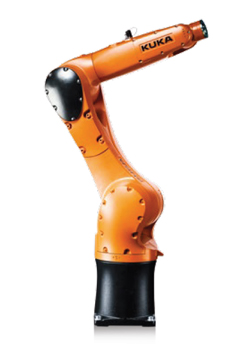
\includegraphics[width=0.7\linewidth]{figures/kuka}
    \caption[test Fig]{This is a test figure. You can use it as a template for your figures}
    \label{fig:kuka}
\end{figure}

%%%%%%%%%%%%%%%%%%%%%%%%%%%%%%%%%%%%%%%%%%%%%%%%%%%%%%%%%%%%%%%%%%%%%%%%%%%%%%%

\setchapterpreamble[o]{%
\dictum[Joseph Addison, \textit{(English essayist, poet, and politician, 1672--1719), Spectator, No. 253}]{% source: http://todayinsci.com/A/Addison_Joseph/AddisonJoseph-Quotations.htm
``It is impossible for us, who live in the latter ages of the world, to make observations in criticism, morality, or in any art or science, which have not been touched upon by others. We have little else left us but to represent the common sense of mankind in more strong, more beautiful, or more uncommon lights.''}\vspace{0.1em}}

\chapter{State of the Art}\label{ch:SotA} %and Related Work
%\input{chapters/relatedWork}
%\input{chapters/stateOfArt}
%%%%%%%%%%%%%%%%%%%%%%%%%%%%%%%%%%%%%%%%%%%%%%%%%%%%%%%%%%%%%%%%%%%%%%%%%%%%%%%

\setchapterpreamble[o]{%
    \dictum[Alan Turing, \textit{(British pioneering computer scientist, cryptanalyst,$\cdots$, and philosopher, 1912--1954)}]{%
        ``A computer would deserve to be called intelligent if it could deceive a human into believing that it was human.''}}
\chapter{Architecture Overview} \label{ch:architecture}
%\input{chapters/architecture.tex}
\cleardoublepage
%\input{chapters/ExperimentalPlatform}
%%%%%%%%%%%%%%%%%%%%%%%%%%%%%%%%%%%%%%%%%%%%%%%%%%%%%%%%%%%%%%%%%%%%%%%%%%%%%%%

\setchapterpreamble[o]{%
  \dictum[Abraham Lincoln, \textit{(American 16$^{th}$ President, 1809--1865)}]{%
    ``Be sure you put your feet in the right place, then stand firm.''}}
\chapter{Robot Foot Ground Contact} \label{ch:legSoilContact}
%\input{chapters/ch2StateOfArt/bekker.tex}
%%%%%%%%%%%%%%%%%%%%%%%%%%%%%%%%%%%%%%%%%%%%%%%%%%%%%%%%%%%%%%%%%%%%%%%%%%%%%%%

\setchapterpreamble[o]{%
  \dictum[Stephen Hawking, \textit{(British theoretical physicist, and cosmologist}]{% source: http://todayinsci.com/A/Addison_Joseph/AddisonJoseph-Quotations.htm
    ``Look up at the stars and not down at your feet. Try to make sense of what you see, and wonder about what makes the universe exist. Be curious.''}}
\chapter{Short--Range Embodied Terrain Classification} \label{ch:shortRange}
%\input{chapters/svm}
%%%%%%%%%%%%%%%%%%%%%%%%%%%%%%%%%%%%%%%%%%%%%%%%%%%%%%%%%%%%%%%%%%%%%%%%%%%%%%%

\setchapterpreamble[o]{%
  \dictum[Chuck Norris, \textit{(American martial artist, actor, film producer and screenwriter)}]{%
    ``I think setting a goal, getting a visual image of what it is you want. You've got to see what it is you want to achieve before you can pursue it.''}}
\chapter{Long--Range Visual Terrain Classification} \label{ch:visual}
%\input{chapters/visualClassification}
%%%%%%%%%%%%%%%%%%%%%%%%%%%%%%%%%%%%%%%%%%%%%%%%%%%%%%%%%%%%%%%%%%%%%%%%%%%%%%%

\setchapterpreamble[o]{%
  \dictum[Dr. Seuss, \textit{(American writer and cartoonist, 1904--1991)}]{%
    ``You have brains in your head. You have feet in your shoes. You can steer yourself in any direction you choose. You're on your own, and you know what you know. And you are the guy who'll decide where to go.''}}
\chapter{Path Planning and Following } \label{ch:path}
%\input{chapters/pathPlanningCameraModel}

%%%%%%%%%%%%%%%%%%%%%%%%%%%%%%%%%%%%%%%%%%%%%%%%%%%%%%%%%%%%%%%%%%%%%%%%%%%%%%%

\setchapterpreamble[o]{%
  \dictum[Richard P. Feynman, \textit{(American theoretical physicist, 1918--1988)}]{%
    ``It doesn't matter how beautiful your theory is, it doesn't matter how smart you are. If it doesn't agree with experiment, it's wrong.''}}
\chapter{Experiments and Results} \label{ch:experiments}
%\input{chapters/expEmbodied}
%\cleardoublepage
%\input{chapters/expPathFollow}
%%%%%%%%%%%%%%%%%%%%%%%%%%%%%%%%%%%%%%%%%%%%%%%%%%%%%%%%%%%%%%%%%%%%%%%%%%%%%%%
\setchapterpreamble[o]{\dictum[George Henry Lewes, \textit{( English philosopher and critic of literature, 1817--1878)}]{The true function of philosophy is to educate us in the principles of reasoning and not to put an end to further reasoning by the introduction of fixed conclusions.}}
\chapter{Conclusions and Future Outlook} \label{ch:conclusion}
%\input{chapters/conclusion}
%\input{chapters/futureWork}

%%%%%%%%%%%%%%%%%%%%%%%%%%%%%%%%%%%%%%%%%%%%%%%%%%%%%%%%%%%%%%%%%%%%%%%%%%%%%%%
%\appendix
%%\chapter{Camera Calibration, Model, and Configurations}\label{ch:cameraModel}
%%\input{chapters/appCameraModel}
%\chapter{Software Description}\label{ch:softwareDescription}
%\input{chapters/appsSoftwareDescription}

%%%%%%%%%%%%%%%%%%%%%%%%%%%%%%%%%%%%%%%%%%%%%%%%%%%%%%%%%%%%%%%%%%%%%%%%%%%%%%%
\backmatter %------------------------------------------------------------------
\cleardoublepage{}
\renewcommand{\nomname}{List of Symbols and Abbreviations}
\markboth{\nomname}{\nomname}\printnomenclature{}
\nocite{*}
\bibliographystyle{apalike}
%\bibliography{myPhDreferences,myPublications}
%\cleardoublepage{}
%\printindex{} %\cleardoublepage{}
\end{document}